% Template for PLoS
% Version 3.1 February 2015
%
% To compile to pdf, run:
% latex plos.template
% bibtex plos.template
% latex plos.template
% latex plos.template
% dvipdf plos.template
%
% % % % % % % % % % % % % % % % % % % % % %
%
% -- IMPORTANT NOTE
%
% This template contains comments intended 
% to minimize problems and delays during our production 
% process. Please follow the template instructions
% whenever possible.
%
% % % % % % % % % % % % % % % % % % % % % % % 
%
% Once your paper is accepted for publication, 
% PLEASE REMOVE ALL TRACKED CHANGES in this file and leave only
% the final text of your manuscript.
%
% There are no restrictions on package use within the LaTeX files except that 
% no packages listed in the template may be deleted.
%
% Please do not include colors or graphics in the text.
%
% Please do not create a heading level below \subsection. For 3rd level headings, use \paragraph{}.
%
% % % % % % % % % % % % % % % % % % % % % % %
%
% -- FIGURES AND TABLES
%
% Please include tables/figure captions directly after the paragraph where they are first cited in the text.
%
% DO NOT INCLUDE GRAPHICS IN YOUR MANUSCRIPT
% - Figures should be uploaded separately from your manuscript file. 
% - Figures generated using LaTeX should be extracted and removed from the PDF before submission. 
% - Figures containing multiple panels/subfigures must be combined into one image file before submission.
% For figure citations, please use "Fig." instead of "Figure".
% See http://www.plosone.org/static/figureGuidelines for PLOS figure guidelines.
%
% Tables should be cell-based and may not contain:
% - tabs/spacing/line breaks within cells to alter layout or alignment
% - vertically-merged cells (no tabular environments within tabular environments, do not use \multirow)
% - colors, shading, or graphic objects
% See http://www.plosone.org/static/figureGuidelines#tables for table guidelines.
%
% For tables that exceed the width of the text column, use the adjustwidth environment as illustrated in the example table in text below.
%
% % % % % % % % % % % % % % % % % % % % % % % %
%
% -- EQUATIONS, MATH SYMBOLS, SUBSCRIPTS, AND SUPERSCRIPTS
%
% IMPORTANT
% Below are a few tips to help format your equations and other special characters according to our specifications. For more tips to help reduce the possibility of formatting errors during conversion, please see our LaTeX guidelines at http://www.plosone.org/static/latexGuidelines
%
% Please be sure to include all portions of an equation in the math environment.
%
% Do not include text that is not math in the math environment. For example, CO2 will be CO\textsubscript{2}.
%
% Please add line breaks to long display equations when possible in order to fit size of the column. 
%
% For inline equations, please do not include punctuation (commas, etc) within the math environment unless this is part of the equation.
%
% % % % % % % % % % % % % % % % % % % % % % % % 
%
% Please contact latex@plos.org with any questions.
%
% % % % % % % % % % % % % % % % % % % % % % % %

\documentclass[10pt,letterpaper]{article}
\usepackage[top=0.85in,left=2.75in,footskip=0.75in]{geometry}

% Use adjustwidth environment to exceed column width (see example table in text)
\usepackage{changepage}

% Use Unicode characters when possible
\usepackage[utf8]{inputenc}

% textcomp package and marvosym package for additional characters
\usepackage{textcomp,marvosym}

% fixltx2e package for \textsubscript
\usepackage{fixltx2e}

% amsmath and amssymb packages, useful for mathematical formulas and symbols
\usepackage{amsmath,amssymb}

% cite package, to clean up citations in the main text. Do not remove.
\usepackage{cite}

% Use nameref to cite supporting information files (see Supporting Information section for more info)
\usepackage{nameref,hyperref}

% line numbers
\usepackage[right]{lineno}

% ligatures disabled
\usepackage{microtype}
\DisableLigatures[f]{encoding = *, family = * }

% rotating package for sideways tables
\usepackage{rotating}

% Remove comment for double spacing
%\usepackage{setspace} 
%\doublespacing

% Text layout
\raggedright
\setlength{\parindent}{0.5cm}
\textwidth 5.25in 
\textheight 8.75in

% Bold the 'Figure #' in the caption and separate it from the title/caption with a period
% Captions will be left justified
\usepackage[aboveskip=1pt,labelfont=bf,labelsep=period,justification=raggedright,singlelinecheck=off]{caption}

% Use the PLoS provided BiBTeX style
\bibliographystyle{plos2015}

% Remove brackets from numbering in List of References
\makeatletter
\renewcommand{\@biblabel}[1]{\quad#1.}
\makeatother

% Leave date blank
\date{}

% Header and Footer with logo
\usepackage{lastpage,fancyhdr,graphicx}
\usepackage{epstopdf}
\pagestyle{myheadings}
\pagestyle{fancy}
\fancyhf{}
\lhead{
\includegraphics[width=2.0in]{PLOS-submission.eps}}
\rfoot{\thepage/\pageref{LastPage}}
\renewcommand{\footrule}{\hrule height 2pt \vspace{2mm}}
\fancyheadoffset[L]{2.25in}
\fancyfootoffset[L]{2.25in}
\lfoot{\sf PLOS}

% Figures
\usepackage{caption}
\usepackage{subcaption}

% Links
\usepackage{hyperref}


%% Include all macros below

\newcommand{\lorem}{{\bf LOREM}}
\newcommand{\ipsum}{{\bf IPSUM}}

%% END MACROS SECTION


\begin{document}
\vspace*{0.35in}

% Title must be 250 characters or less.
% Please capitalize all terms in the title except conjunctions, prepositions, and articles.

% A fine-scale, process-based, dynamic landscape evolution model

\begin{flushleft}
{\Large
\textbf\newline{Dynamic Landscape Evolution}
}
\newline
% Insert author names, affiliations and corresponding author email (do not include titles, positions, or degrees).
\\
Brendan Alexander Harmon\textsuperscript{1,2,*},
Helena Mitasova\textsuperscript{1,3},
Vaclav Petras\textsuperscript{1,3},
Anna Petrasova\textsuperscript{1,3}
\\
\bigskip
\bf{1} Center for Geospatial Analytics, North Carolina State University, Raleigh, North Carolina, United States of America
\\
\bf{2} Department of Landscape Architecture, North Carolina State University, Raleigh, North Carolina, United States of America
\\
\bf{3} Department of Marine, Earth, and Atmospheric Sciences, North Carolina State University, Raleigh, North Carolina, United States of America
\\
\bigskip

% Insert additional author notes using the symbols described below. Insert symbol callouts after author names as necessary.
% 
% Remove or comment out the author notes below if they aren't used.
%
% Primary Equal Contribution Note
%\Yinyang These authors contributed equally to this work.

% Additional Equal Contribution Note
% Also use this double-dagger symbol for special authorship notes, such as senior authorship.
%\ddag These authors also contributed equally to this work.

% Current address notes
%\textcurrency a Insert current address of first author with an address update
% \textcurrency b Insert current address of second author with an address update
% \textcurrency c Insert current address of third author with an address update

% Deceased author note
%\dag Deceased

% Group/Consortium Author Note
%\textpilcrow Membership list can be found in the Acknowledgments section.

% Use the asterisk to denote corresponding authorship and provide email address in note below.
* baharmon@ncsu.edu

\end{flushleft}
% Please keep the abstract below 300 words
\section*{Abstract}

This is a fine-scale, short term, process-based landscape evolution model using simulated erosion and deposition to generate a timeseries of digital elevation models. This model uses a path sampling method to solve water and sediment flow continuity equations and model mass flows over complex topographies based on topographic, land cover, soil, and rainfall parameters. This either steady state or dynamic model can simulate landscape evolution for a range of hydrologic soil erosion regimes. 
%The change in elevation is a function of time, net erosion-deposition, and sediment mass density.



\linenumbers

\section*{Introduction}

%With process-based simulations we have procedurally modeled how a landscape could evolve as the flow of water erodes the landscape surface and shapes its terrain.
This process-based, spatial distributed, dynamic model uses a path sampling method to solve the water and sediment flow equations
\cite{mitasova2004}
and model mass flows over complex topographies based on topographic, land cover, soil, and rainfall parameters.
The modeled flow of sediment -- a function of the flow of water, soil detachment, and transport parameters -- is then used to estimate the net erosion and deposition rates and the associated short-term evolution of the topography.


\subsection*{Shallow water flow}

We simulated shallow overland water flow controlled by spatially variable topography, soil, landcover, and rainfall parameters using the SIMWE model to solve the continuity and momentum equations for steady state water flow with a path sampling method. 
% implemented in GRASS GIS as the module r.sim.water.
%
Shallow water flow can be approximated by
the bivariate form of the St Venant equation:

\begin{equation}
\label{eq:water}
{\partial h({\bf r},t) \over \partial t} =
 i_e({\bf r},t) - \nabla \cdot {\bf q}({\bf r},t)
\end{equation}

where:

\hspace*{1em} ${\bf r}(x,y)$ is the position [m]

\hspace*{1em} $t$ is the time [s]

\hspace*{1em} $h({\bf r},t)$ is the depth of overland flow [m]

\hspace*{1em} $i_e({\bf r},t)$ is the rainfall excess [m/s]\\
\hspace*{1em} (rainfall $-$ infiltration $-$ vegetation intercept) 

\hspace*{1em} ${\bf q}({\bf r},t)$ is the water flow per unit width [$\rm m^2/s$].

%  diffusion wave approximation
By integrating a diffusion term $ \propto \nabla^2 [h^{5/3}({\bf r})]$ 
into
the solution of the continuity and momentum equations for steady state water flow
diffusive wave effects can be approximated
so that water can flow through depressions. 
%
\begin{equation}
\label{eq:difwater}
-{\varepsilon({\bf r})\over 2 }\nabla^2 [h^{5/3}({\bf r})]
+\nabla \cdot [ h({\bf r}){\bf v}({\bf r})] = i_e({\bf r})
\end{equation}

 where:
 
 \hspace*{1em} $\varepsilon({\bf r})$ is a spatially variable diffusion coefficient.

This equation is solved using a Green's function Monte Carlo path sampling method \cite{mitasova2004}.

%Steady state water flow equation with a 2D diffusive wave approximation\ldots

%continuity and momentum equations for a steady water flow with a diffusive wave approximation



\subsection*{Sediment flow}

Steady state sediment flow equation with diffusion\ldots
\begin{equation}\label{eq:sediment} 
...
\end{equation}


\subsection*{Landscape evolution}


Detachment limited landscape evolution

\begin{equation}\label{eq:flux_evolution} 
{\Delta z(x,y,t) = \Delta t \cdot q_s(x,y,t) \cdot \varrho(r)^{-1} }
\end{equation}

where: 

$\Delta z =$ change in elevation $(m)$ \\
$q_s =$ sediment flux $(kg \cdot m^{-1} s^{-1})$ \\
$\varrho =$ mass of water carried sediment per unit area $(kg \cdot m^{-2})$ \\
\vspace{1em}

Transport capacity limited landscape evolution

%change in elevation (m) = change in time (s) * net erosion-deposition (kg/m^2s) / sediment mass density (kg/m^3)
\begin{equation}\label{eq:evolution} 
{\Delta z(x,y,t) = \Delta t \cdot d_s(x,y,t) \cdot \rho_s^{-1} }
\end{equation}

where: 

$\Delta z =$ change in elevation $(m)$ \\
$d_s =$ net erosion-deposition $(kg ~ m^{-2} s^{-1})$ \\
$\rho_s =$ sediment mass density $(kg ~m^{-3})$ \\
\vspace{1em}

\ldots
\cite{mitasova2013}





\section*{Methods}

\subsection*{Implementation}

\begin{enumerate}
\item Function for sediment flux based landscape evolution
\item Function for erosion-deposition based landscape evolution
\item Function for dynamic modeling based on constant parameters
\item Function for dynamic modeling based on list of rainfall observations
\item Registration in temporal framework
\item Handling of edge effects from moving window computations
\end{enumerate}

This set of python scripts is available on Github at \url{https://github.com/baharmon/landscape_evolution} released under the GNU General Public License version 2. These scripts are meant to be run inside of GRASS GIS using the GRASS Python Scripting Library. GRASS GIS is an open source project released under the GNU General Public License version 2. GRASS GIS is available at \url{https://grass.osgeo.org/}. 

\subsection*{Tangible landscape evolution}

Tangible Landscape -- a tangible user interface tightly integrated with a geographic information system for intuitively sketching in 3D \cite{petrasova2015}. Conceptually, Tangible Landscape couples a physical model with a digital model in a real-time feedback cycle of 3D scanning, geospatial modeling and simulation, and projection in order to physically manifest digital data as tangible bits. With tangible bits users can directly, physically feel and manipulate data with their bodies -- naturally, intuitively understanding space, form, and process. Tangible Landscape is available on Github at \url{https://github.com/ncsu-osgeorel/grass-tangible-landscape}.

%\paragraph{Testing}
We coupled Tangible Landscape with the landscape evolution model to test the model and experiment with strategies for restoration. 
We used Tangible Landscape to computational steer the landscape evolution model and interactively explore the relationship between overland flow patterns and changes in topography. By manually changing the physical model of the landscape 
we change the topography used by the model.

\begin{figure}
\centering
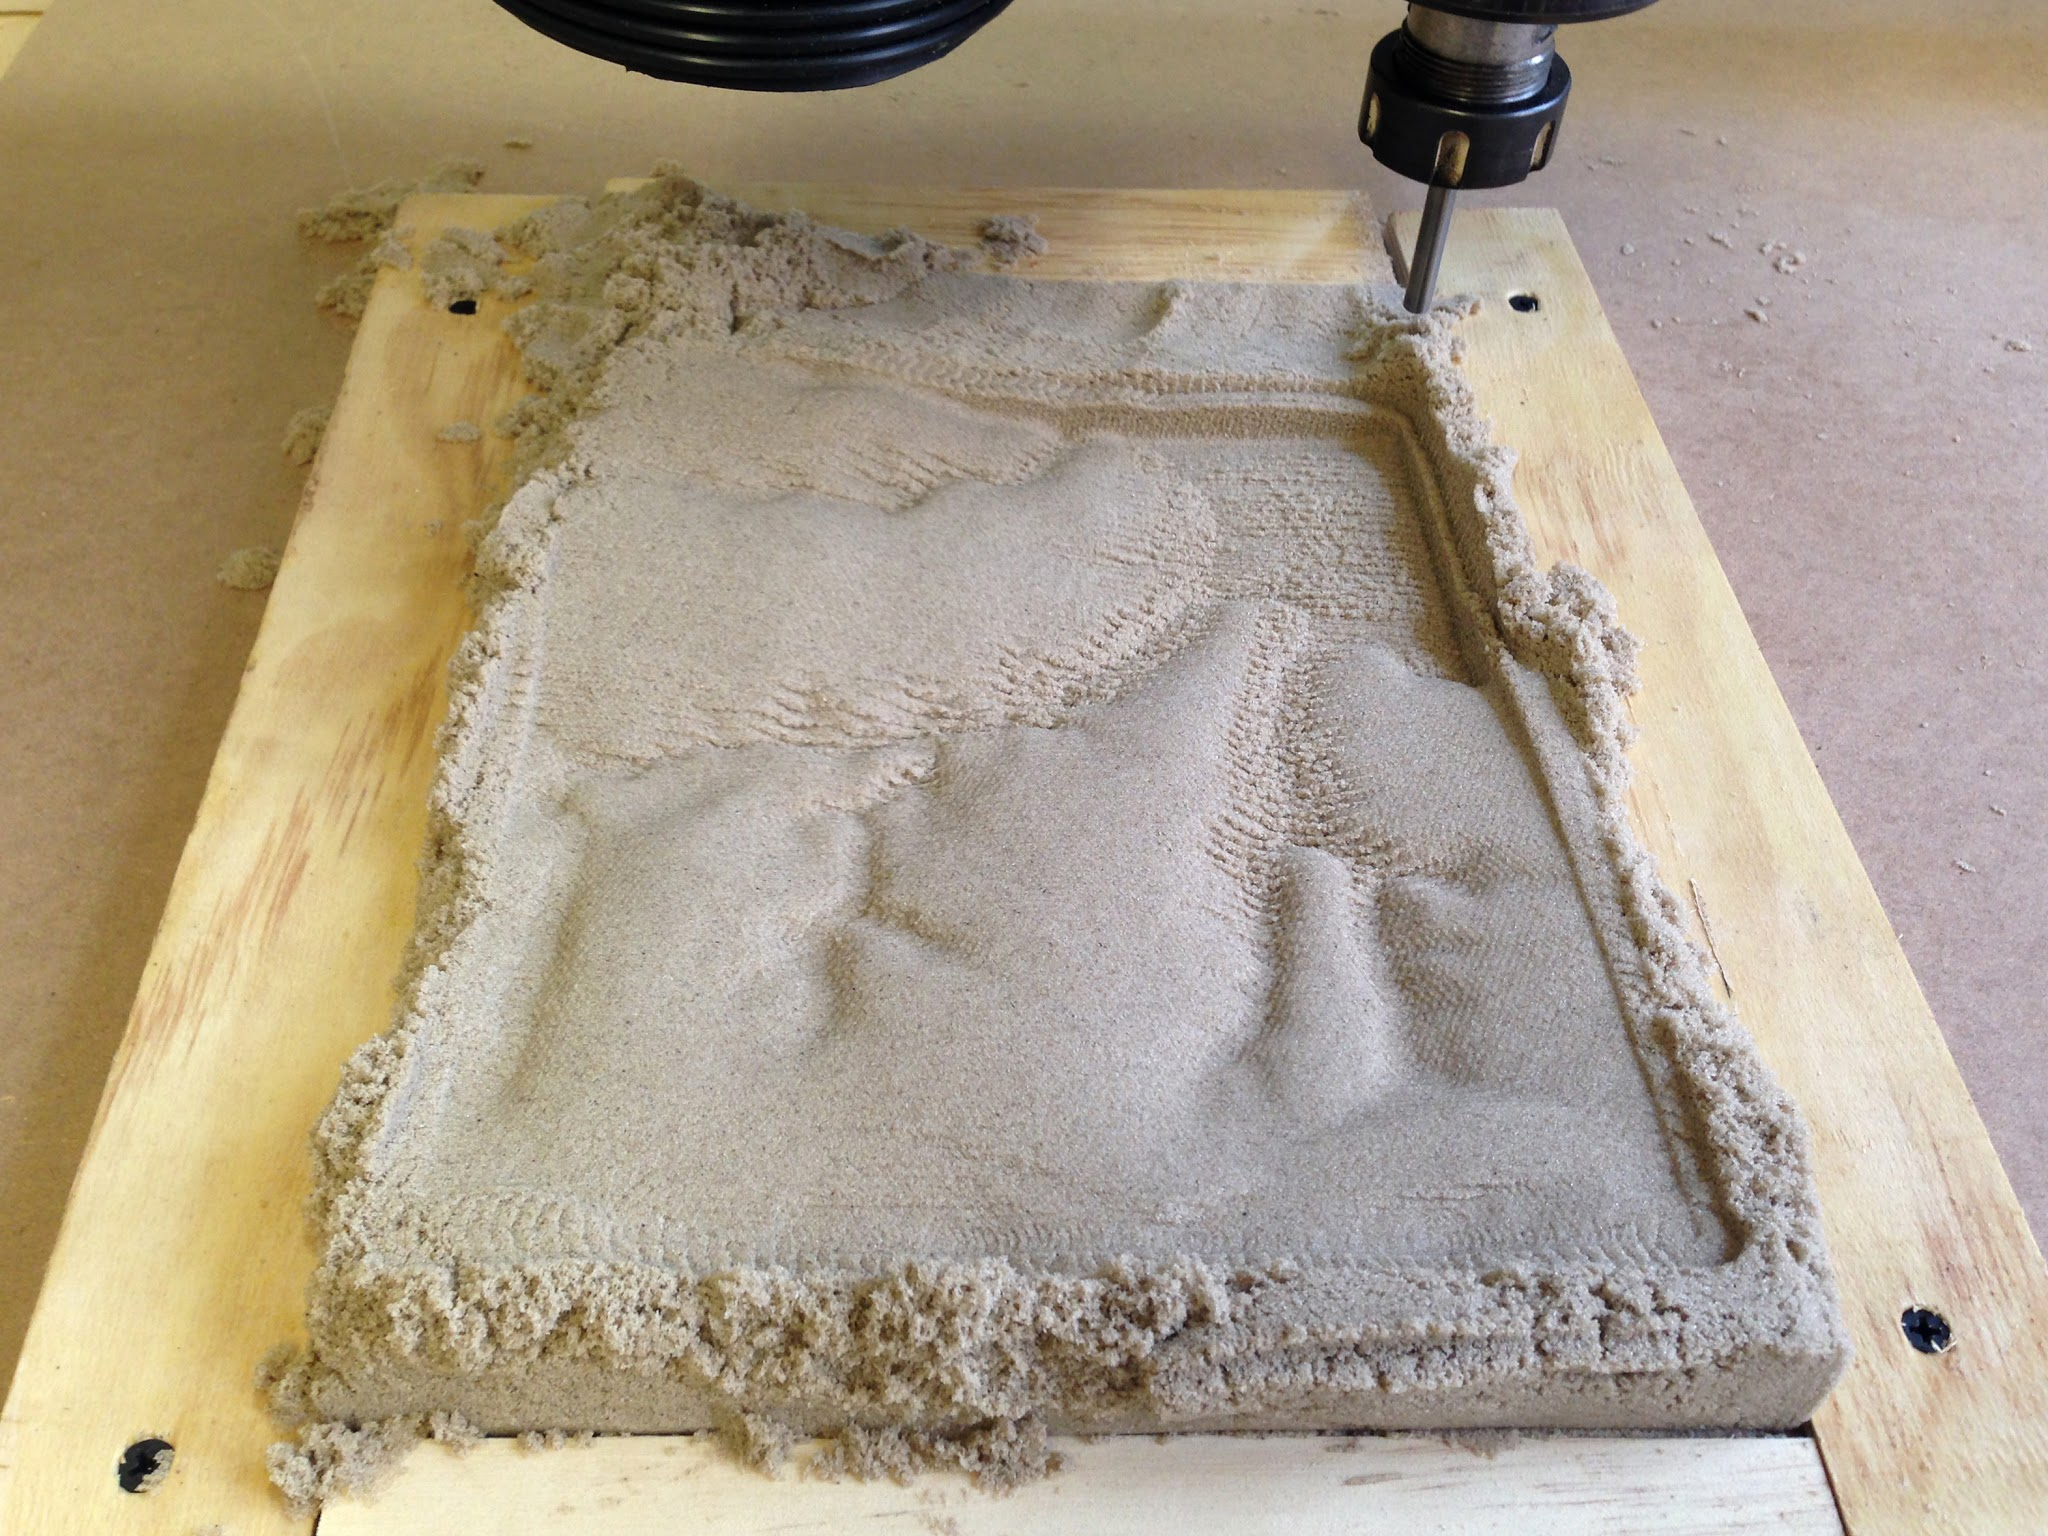
\includegraphics[width=\textwidth]{images/cnc_sand.jpg}
\caption{{\bf Rapid prototyping.}
3-axis CNC fabrication of the evolved landscape in polymer-enriched sand using a plunge cut.}
\label{fig:cnc_sand}
\end{figure}




\section*{Results}

\begin{figure}
\centering
%   
\begin{subfigure}[b]{0.3\textwidth}
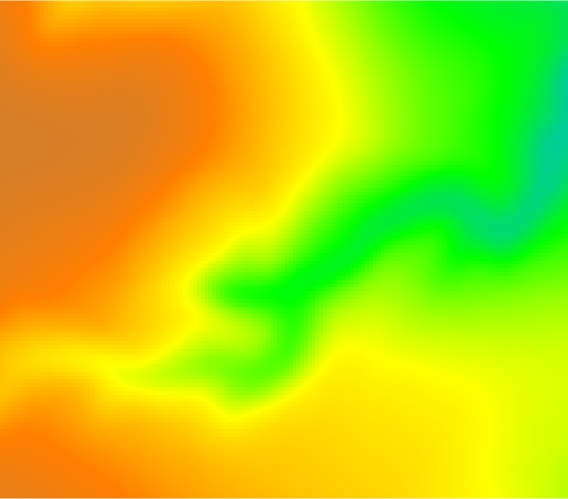
\includegraphics[width=\textwidth]{images/lrwoods_elevation.png}
%[trim={0 0 0 1cm},clip,width=\textwidth]
\label{fig_1_1}
\textbf{a} \\
\end{subfigure}
%
~ %add desired spacing between images, e. g. ~, \quad, \qquad, \hfill etc.
%
\begin{subfigure}[b]{0.3\textwidth}
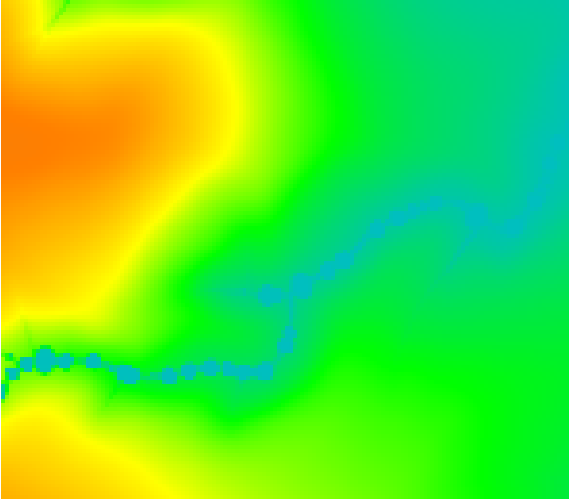
\includegraphics[width=\textwidth]{images/lrwoods_dynamics_flux_5m_30m.png}
\label{fig_1_2}
\textbf{b} \\
\end{subfigure}
%
~ %add desired spacing between images, e. g. ~, \quad, \qquad, \hfill etc.
%
\begin{subfigure}[b]{0.3\textwidth}
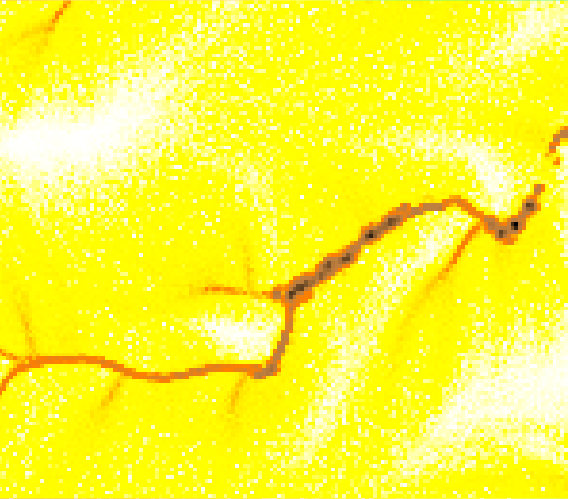
\includegraphics[width=\textwidth]{images/lrwoods_dynamics_erdep_5m_30m_flux.png} % REPLACE IMAGE
\label{fig_1_3}
\textbf{c} \\
\end{subfigure}
%
\caption{{\bf Sediment flux based gully evolution.}
\textbf{a)}
A bare earth digital elevation model of gully in Lake Raleigh Woods, North Carolina derived from lidar data.
\textbf{b)}
The simulated evolution of the gully based on a detachment limited soil erosion regime.
The landscape evolution model was run as a dynamic simulation with 155 mm/hr rainfall intensity for 5 minutes intervals over a 30 min period.
This run of model carved deep pits along the center of the channel.
\textbf{c)}
Simulated sediment flux. 
}
\label{fig_1}
\end{figure}



\begin{figure}
\centering
%   
\begin{subfigure}[b]{0.3\textwidth}
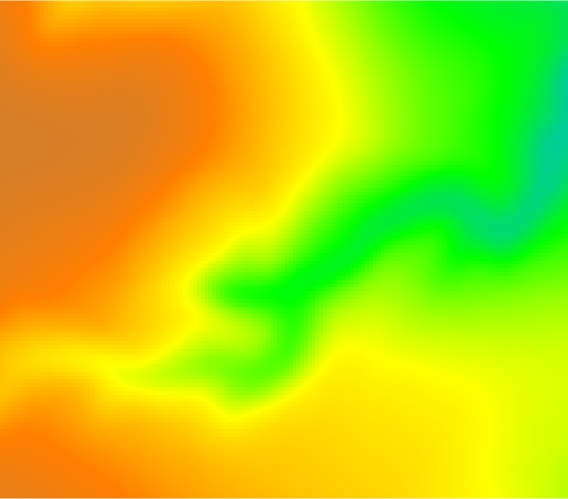
\includegraphics[width=\textwidth]{images/lrwoods_elevation.png}
%[trim={0 0 0 1cm},clip,width=\textwidth]
\label{fig_2_1}
\textbf{a} \\
\end{subfigure}
%
~ %add desired spacing between images, e. g. ~, \quad, \qquad, \hfill etc.
%
\begin{subfigure}[b]{0.3\textwidth}
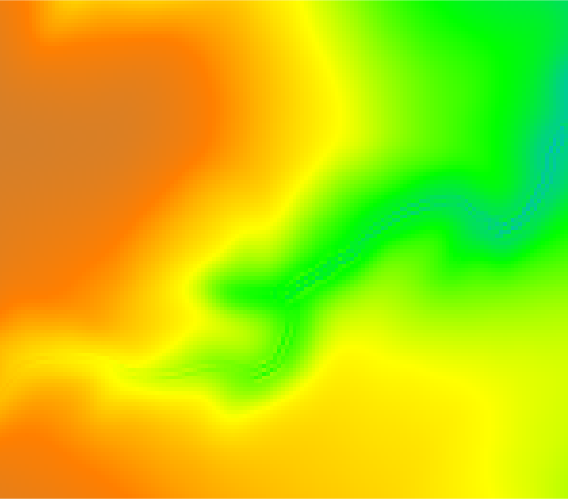
\includegraphics[width=\textwidth]{images/lrwoods_dynamics_erdep_5m_30m.png}
\label{fig_2_2}
\textbf{b} \\
\end{subfigure}
%
~ %add desired spacing between images, e. g. ~, \quad, \qquad, \hfill etc.
%
\begin{subfigure}[b]{0.3\textwidth}
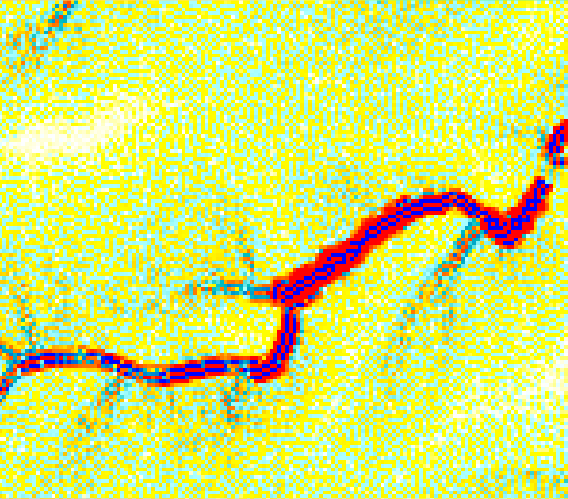
\includegraphics[width=\textwidth]{images/lrwoods_dynamics_erdep_5m_30m_erdep.png} % REPLACE IMAGE
\label{fig_2_3}
\textbf{c} \\
\end{subfigure}
%
\caption{{\bf Erosion - deposition based gully evolution.}
\textbf{a)}
A bare earth digital elevation model of gully in Lake Raleigh Woods, North Carolina derived from lidar data.
\textbf{b)}
The simulated evolution of the gully based on a transport capacity limited  soil erosion regime.
The landscape evolution model was run as a dynamic simulation with 155 mm/hr rainfall intensity for 5 minutes intervals over a 30 min period.
This run of model carved a deeper channel, accumulated deposited sediment along the centerline of the channel, and accumulated deposited sediments along the banks of the channel.
\textbf{c)}
Simulated erosion-deposition. 
}
\label{fig_1}
\end{figure}





\begin{figure}
\centering
%   
\begin{subfigure}[b]{0.4\textwidth}
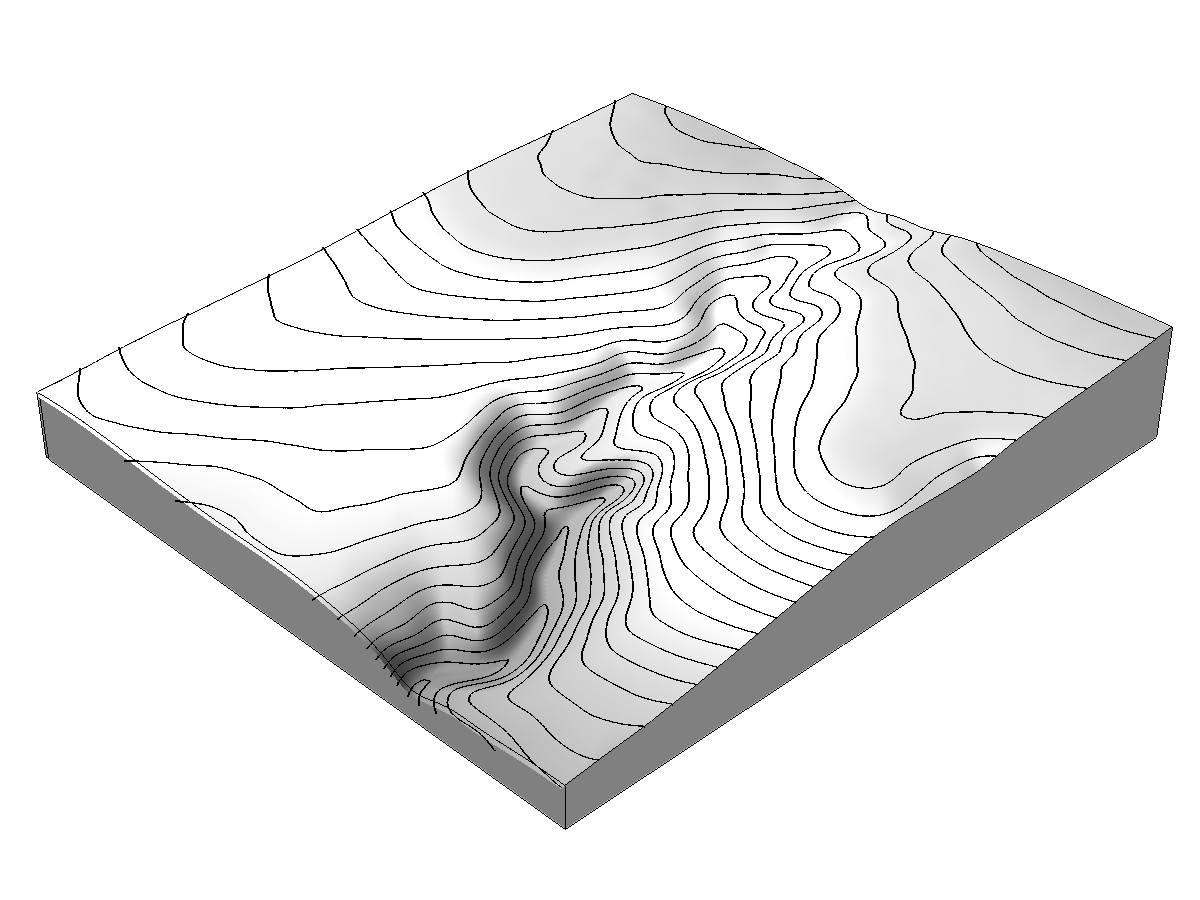
\includegraphics[width=\textwidth]{images/dem.png}
%[trim={0 0 0 1cm},clip,width=\textwidth]
\label{fig_2_1}
\textbf{a} \\
\end{subfigure}
%
~ %add desired spacing between images, e. g. ~, \quad, \qquad, \hfill etc.
%
\begin{subfigure}[b]{0.4\textwidth}
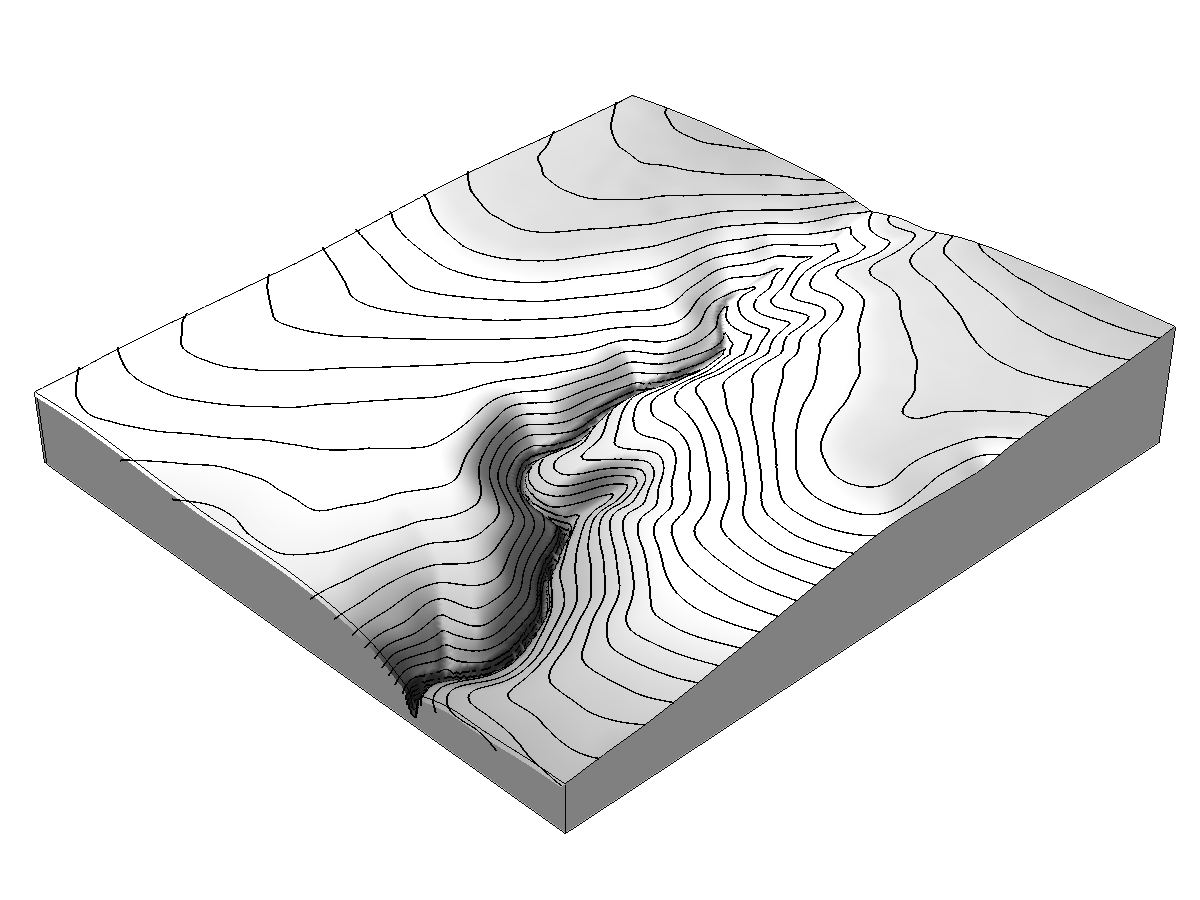
\includegraphics[width=\textwidth]{images/evolved_dem.png}
\label{fig_2_2}
\textbf{b} \\
\end{subfigure}
%
\caption{{\bf Sediment flux based gully evolution.}
\textbf{a)}
A gully in Lake Raleigh Woods, North Carolina.
\textbf{b)}
The simulated evolution of the gully based on a detachment limited soil erosion regime. 
The landscape evolution model was run as a steady state simulation with 155 mm/hr rainfall intensity for 10 minutes to model a 10-year storm event. 
This run of the model carved a deep incision along the centerline of the channel.
}
\label{fig_2}
\end{figure}




\begin{figure}
\centering
%   
\begin{subfigure}[b]{0.4\textwidth}
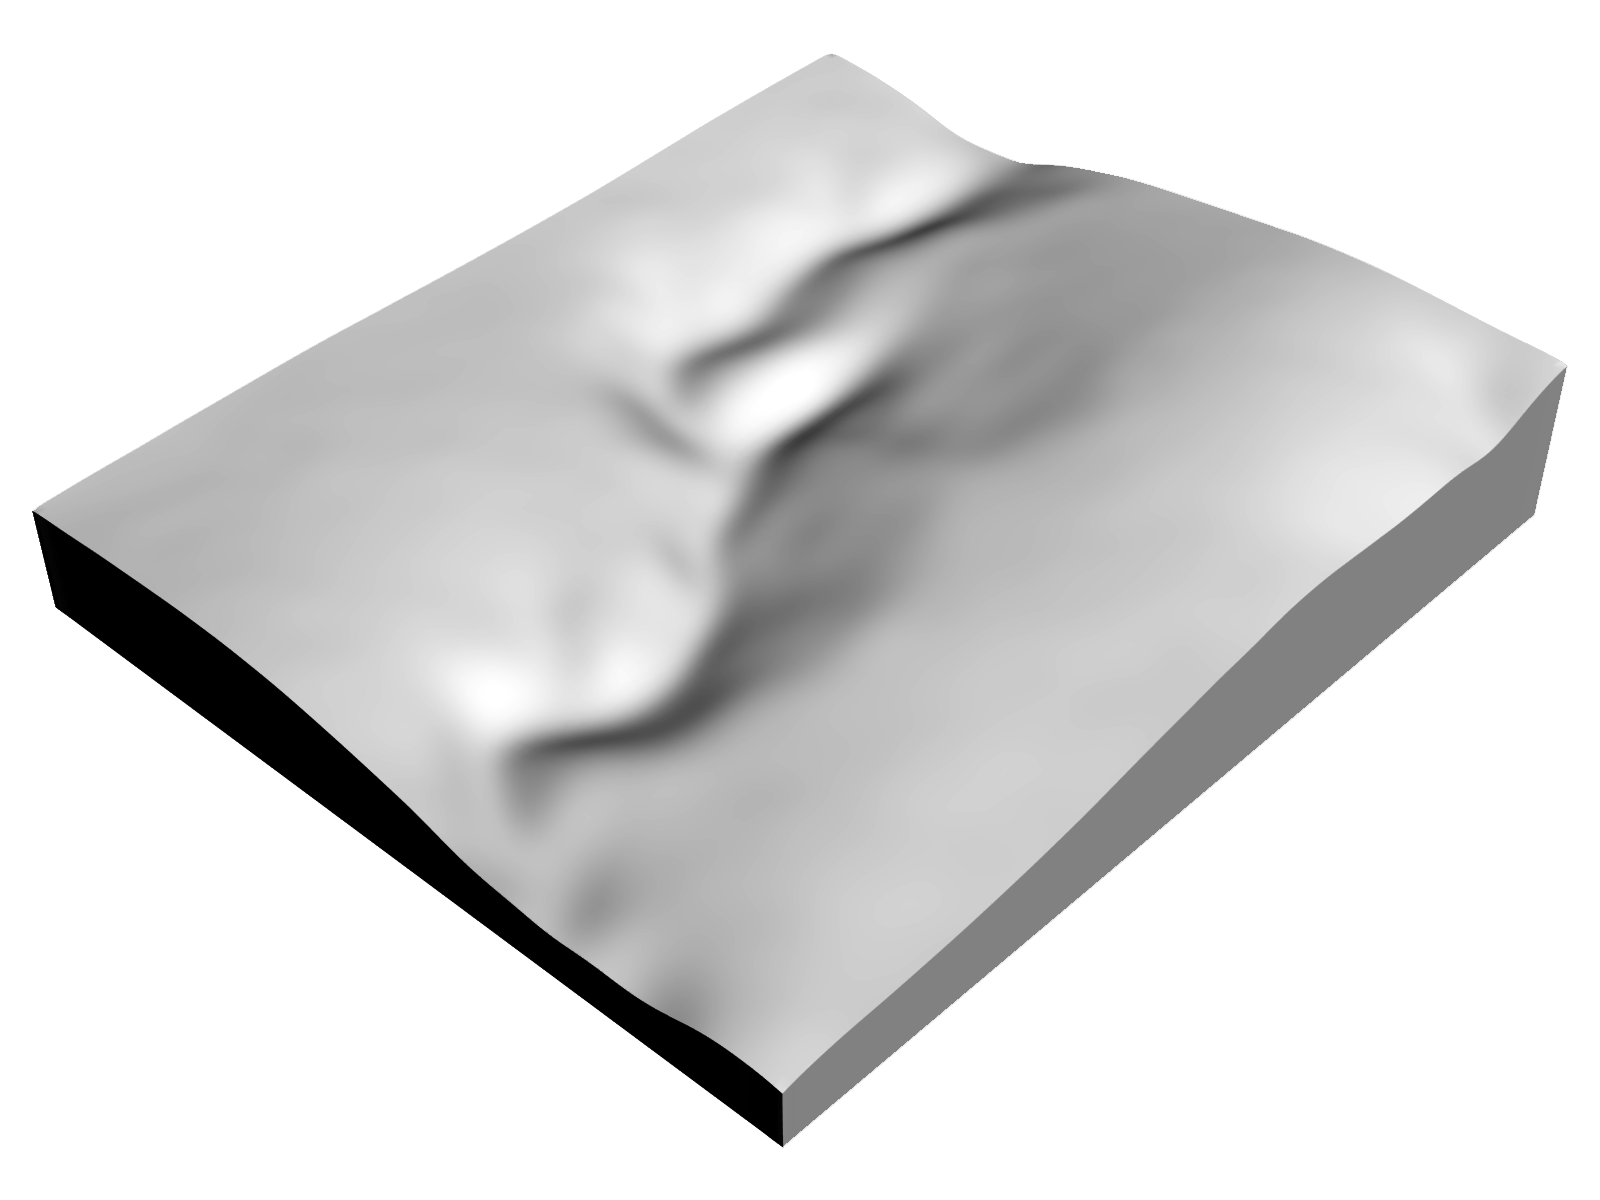
\includegraphics[width=\textwidth]{images/elevation_render.png}
%[trim={0 0 0 1cm},clip,width=\textwidth]
\label{fig_3_1}
\textbf{a} \\
\end{subfigure}
%
~ %add desired spacing between images, e. g. ~, \quad, \qquad, \hfill etc.
%
\begin{subfigure}[b]{0.4\textwidth}
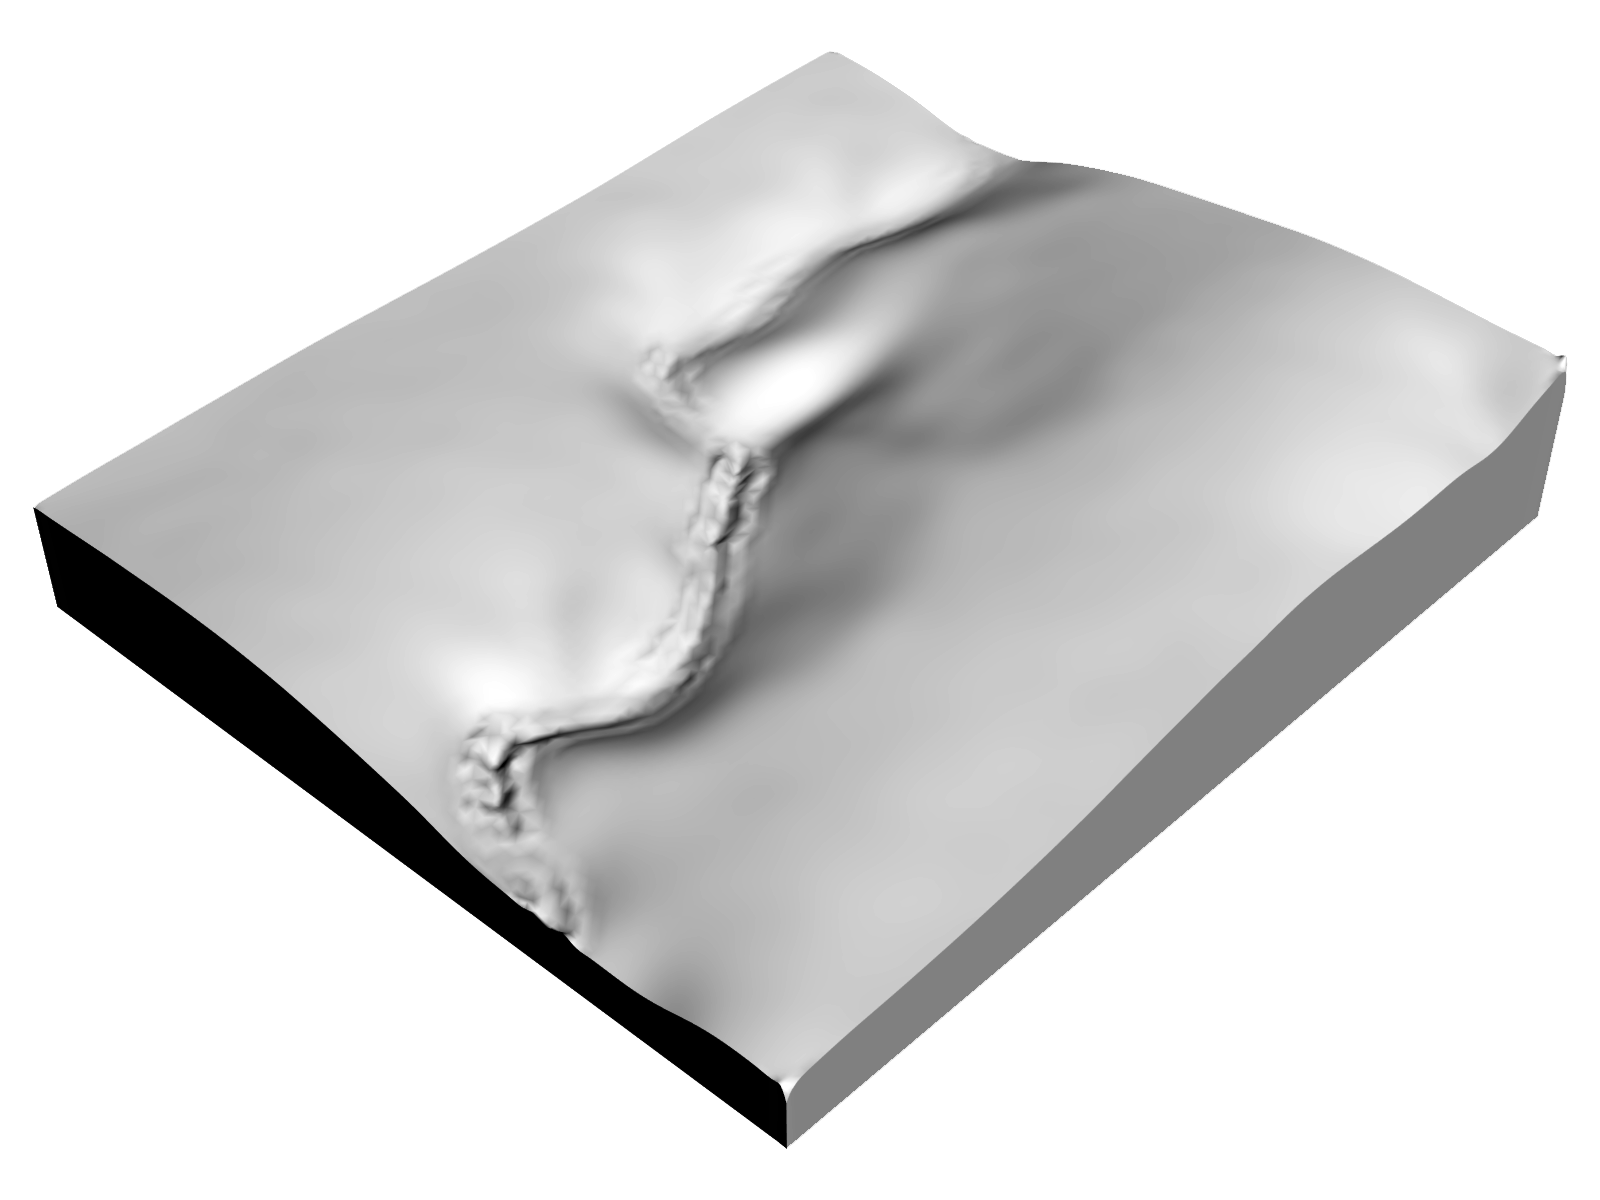
\includegraphics[width=\textwidth]{images/evolved_elevation_render.png}
\label{fig_3_2}
\textbf{b} \\
\end{subfigure}
%
\caption{{\bf Erosion-deposition based gully evolution.}
\textbf{a)}
A gully in Lake Raleigh Woods, North Carolina.
\textbf{b)}
The simulated evolution of the gully based on a transport capacity limited  soil erosion regime.
The landscape evolution model was run as a dynamic simulation with 155 mm/hr rainfall intensity for 5 minutes intervals over a 30 min period.
This run of model carved a deeper channel, accumulated deposited sediment along the centerline of the channel, and accumulated deposited sediments along the banks of the channel.
}
\label{fig_3}
\end{figure}



\section*{Discussion}

\subsection*{Future work}
\begin{enumerate}
\item Add water and suspended sediment particles to next run
\item Test the model on historical data
\item Test the model with field data
\item Empirically calibrate the parameters
\item Refactor code
\item Develop a GRASS GIS addon
\item Implement as a Tangible Landscape analysis
\item Live, in-situ fabrication in polymer-enriched sand with a robotic arm
\end{enumerate}


\section*{Supporting Information}

\subsection*{S1 File.}
\label{S1_File}
{\bf Python scripts.}
(ZIP)

\subsection*{S2 File.}
\label{S2_File}
{\bf GIS data.}
(ZIP)

%\section*{Acknowledgments}
%\ldots

%\begin{figure}[h]
%\centering
%\includegraphics[width=\textwidth]{images/}
%\caption{{\bf Figure Title \ldots .}
%Figure Caption \ldots .}
%\label{fig1}
%\end{figure}


%% For figure citations, please use "Fig." instead of "Figure".
%Fig.~\ref{fig1} 
%
%~\cite{bib1}
%
%Eq.~(\ref{eq:1}) 
%
%%Table~\ref{table1}
%
%\nameref{S1_Video} 
%
%\begin{figure}[h]
%\caption{{\bf Figure Title \ldots .}
%Figure Caption \ldots .}
%\label{fig1}
%\end{figure}
%
%\begin{enumerate}
%\item{\ldots}
%\item{\ldots}
%\item{\ldots}
%\end{enumerate}
%
%% For 3rd level headings, use \paragraph{}. 



\nolinenumbers

\nocite{*}

\bibliography{landscape_evolution.bib}

%\section*{References}

% Either type in your references using
% \begin{thebibliography}{}
% \bibitem{}
% Text
% \end{thebibliography}
%
% OR
%
% Compile your BiBTeX database using our plos2015.bst
% style file and paste the contents of your .bbl file
% here.
% 

%\begin{thebibliography}{10}
%
%\bibitem{bib1}
%Devaraju P, Gulati R, Antony PT, Mithun CB, Negi VS. Susceptibility to SLE in South Indian Tamils may be influenced by genetic selection pressure on TLR2 and TLR9 genes. Mol Immunol. 2014 Nov 22. pii: S0161-5890(14)00313-7. doi: 10.1016/j.molimm.2014.11.005
%
%\bibitem{bib2}
%Huynen MMTE, Martens P, Hilderlink HBM. The health impacts of globalisation: a conceptual framework. Global Health. 2005;1: 14. Available: http://www.globalizationandhealth.com/content/1/1/14.
%
%\end{thebibliography}



\end{document}

